\section{Pianificazione dei test}
\label{pianificazioneDeiTest}
Di seguito verranno descritti tutti i test di integrazione, sistema e validazione che il gruppo \authorName{} intende effettuare. È previsto un futuro aggiornamento per quanto riguarda i test di unità. Nel \PdP{} vengono specificate le tempistiche di esecuzione dei test.\\
Nelle tabelle sottostanti la colonna dello \textit{Stato} dei test riporterà il valore \textbf{N.I.} per i test che devono ancora essere effettuati; essi verranno eseguiti successivamente, come descritto nel \PdP{}.  

\subsection{Test di sistema}
\label{testdisistema}
In questa sezione vengono descritti i test di sistema, il cui obbiettivo è quello di verificare il comportamento dinamico dell'intero sistema, rispetto ai requisiti descritti nel documento \textit{Analisi dei Requisiti v4.0.0}.
Vengono qui di seguito riportati i test di sistema ritenuti meritevoli di un test, al fine di garantire il soddisfacimento dei requisiti software individuati.

\subsubsection{Descrizione test di sistema}
\label{descrizionetestdisistema}	

\newdimen\larghezza
\setlength{\larghezza}{7cm}
\newdimen\dimTipo
\setlength{\dimTipo}{2cm}
\newdimen\dimFonti
\setlength{\dimFonti}{2cm}
	

\begin{center}
\begin{longtable}[!h]{|c|c|c|c|}
\hline



\textbf{Test} & \textbf{Descrizione} & \textbf{Stato} & \textbf{Requisito} \\


\hline
TS1.2.1.1 & \parbox[t]{\larghezza}{Viene verificato che il sistema accetti in input file di formato PNG}  & superato & R0F1.2.1.1 \\ 
\hline
TS1.2.1.2 & \parbox[t]{\larghezza}{Viene verificato che il sistema accetti in input file di formato JPG}  & superato & R0F1.2.1.2 \\ 
\hline
TS1.2.1.3 & \parbox[t]{\larghezza}{Viene verificato che il sistema accetti in input file di formato BMP}  & superato & R0F1.2.1.3 \\ 
\hline
TS1.2.1.4 & \parbox[t]{\larghezza}{Viene verificato che il sistema accetti in input file di formato AVI}  & superato & R0F1.2.1.4 \\ 
\hline
TS1.2.1.5 & \parbox[t]{\larghezza}{Viene verificato che il sistema accetti in input file di formato NIfTI}  & superato & R0F1.2.1.5 \\ 
\hline
TS1.2.1.6 & \parbox[t]{\larghezza}{Viene verificato che il sistema accetti in input file di formato Analyze7.5}  & superato & R0F1.2.1.6 \\ 
\hline
TS1.3.1 & \parbox[t]{\larghezza}{Viene verificato che il sistema accetti in input file di formato PNG per le maschere }  & superato & R0F1.3.1 \\ 
\hline
TS1.3.2 & \parbox[t]{\larghezza}{Viene verificato che il sistema accetti in input file di formato JPG per le maschere }  & superato & R0F1.3.2 \\ 
\hline
TS1.3.3 & \parbox[t]{\larghezza}{Viene verificato che il sistema accetti in input file di formato BMP per le maschere }  & superato & R0F1.3.3 \\ 
\hline
TS1.3.4 & \parbox[t]{\larghezza}{Viene verificato che il sistema accetti in input file di formato NIfTI per le maschere }  & superato & R0F1.3.4 \\ 
\hline
TS1.3.5 & \parbox[t]{\larghezza}{Viene verificato che il sistema accetti in input file di formato Analyze7.5 per le maschere }  & superato & R0F1.3.5 \\ 
\hline
TS1.4 & \parbox[t]{\larghezza}{Viene verificato che il sistema visualizzi correttamente un errore quando si cerca di caricare un immagine di formato non consentito}  & N.I. & R0F1.4 \\ 
\hline
TS10.2.1 & \parbox[t]{\larghezza}{Viene verificato che il software,se richiesto, mostri il risultato delle features appena processate}  & superato & R0F10.2.1 \\ 
\hline
TS12.2 & \parbox[t]{\larghezza}{Viene verificato che i risultati delle analisi effettuate vengano esportati nel formato corretto}  & superato & R0F12.2 \\ 
\hline
TS13.1 & \parbox[t]{\larghezza}{Viene verificato che vengano visualizzate correttamente le immagini 2D all'interno del software}  & superato & R0F13.1 \\ 
\hline
 TS13.2 & \parbox[t]{\larghezza}{Viene verificato che vengano visualizzate correttamente le immagini 3D all'interno del software}  & superato & R0F13.2 \\ 
\hline
TS16 & \parbox[t]{\larghezza}{Viene verificato che il sistema funzioni su Windows 7 32bit senza service pack o superiore}  & superato & R0V16 \\ 
\hline
TS17 & \parbox[t]{\larghezza}{Viene verificato che il sistema funzioni su Windows 7 64bit senza service pack o superiore}  & superato & R0V17 \\ 
\hline
TS18 & \parbox[t]{\larghezza}{Viene verificato che il sistema funzioni su Ubuntu 12.04 32bit o superiore}  & superato & R0V18 \\ 
\hline
TS19 & \parbox[t]{\larghezza}{Viene verificato che il sistema funzioni su Ubuntu 12.04 64bit o superiore}  & superato & R0V19 \\ 
\hline
 TS20 & \parbox[t]{\larghezza}{Viene verificato che il sistema funzioni su Mac OS X 10.9 o superiore}  & N.I. & R0V20 \\ 
\hline
TS21 & \parbox[t]{\larghezza}{Viene verificato che i risultati vengano visualizzati senza perdita di qualità}  & superato & R0V21 \\ 
\hline
\caption{Tracciamento test di sistema-requisiti}
\end{longtable}
\end{center}

\subsection{Test di integrazione}
\label{test_integrazione}
In questa sezione vengono descritti i test di integrazione, necessari per verificare che il comportamento di più unità combinate sia corretto.
L'approccio utilizzato è di tipo \textit{bottom-up}, che consiste nell'integrare prima le unità a livello più basso, ossia quelle che rappresentano la logica di base del sistema e in seguito quelle ai livelli superiori. Le unità base, conosciute anche come \textit{moduli di unità}, si riferiscono ai requisiti obbligatori e quindi alle funzionalità più importanti del sistema. Adottando questo tipo di approccio, è quindi possibile verificare più volte il comportamento di queste unità, massimizzando la ricerca di eventuali errori presenti.
Il diagramma seguente non rispetta il formalismo UML ma specifica graficamente la strategia d'integrazione adottata.

\begin{figure}[!h]
		\centering
		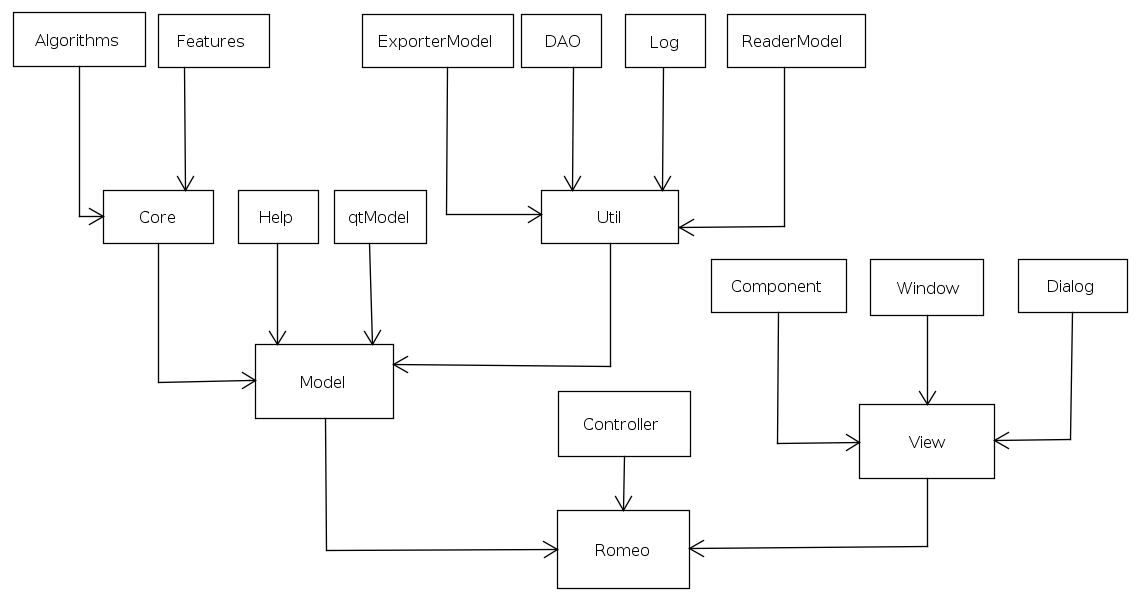
\includegraphics[scale=0.5]{./img/Integrazione}
		\caption{Diagramma informale della strategia di integrazione}
	\end{figure}

\newdimen\larghezza
\setlength{\larghezza}{7cm}
\newdimen\dimTipo
\setlength{\dimTipo}{2cm}
\newdimen\dimFonti
\setlength{\dimFonti}{2cm}
	
\begin{center}
\begin{longtable}{|c|c|c|c|}
\hline

\textbf{Test} & \textbf{Descrizione} & \textbf{Componente} & \textbf{Stato} \\


\hline
TI-Algorithms & \parbox[t]{\larghezza}{\textbf{Algoritmi di clustering:} verificare la presenza di tutti gli algoritmi di clustering definiti nei requisti}  & Algorithms & Superato \\ 
\hline
TI-Component & \parbox[t]{\larghezza}{\textbf {Componenti grafici delle finestre:} verifica la corretta visualizzazione e responsività dei menù nelle finestre del sistema}  & Component & Superato \\ 
\hline
TI-Core & \parbox[t]{\larghezza}{\textbf {Core del sistema:} verifica il corretto funzionamento delle operazioni di analisi}  & Core & Superato \\ 
\hline
TI-DAO & \parbox[t]{\larghezza}{\textbf {Interfaccia Database:} verifica la corretta interazione del sistema con il database}  & DAO & Superato \\ 
\hline
TI-Dialog & \parbox[t]{\larghezza}{\textbf {Sistema di dialogo con l'utente:} verifica il corretto funzionamento delle finestre di dialogo con l'utente}  & Dialog & Superato \\ 
\hline
TI-ExporterModel & \parbox[t]{\larghezza}{\textbf {Sistema di esportazione:} verifica che le immagini vengano esportate correttamente}  & ExporterModel & Superato \\ 
\hline
TI-Features & \parbox[t]{\larghezza}{\textbf{Feature Extractor:} verificare la presenza di tutte le feature extractor definite nei requisti}  & Features & Superato \\ 
\hline
TI-Help & \parbox[t]{\larghezza}{\textbf {Sistema d'aiuto:} verifica il corretto funzionamento delle operazioni del sistema di aiuto}  & Help & Superato \\ 
\hline
TI-Log & \parbox[t]{\larghezza}{\textbf {Sistema di log:} verifica che venga creato un file di testo che riporta tutte le operazioni compiute dal sistema}  & Log & Superato \\ 
\hline
TI-Model & \parbox[t]{\larghezza}{\textbf {Logica di Business:}  viene verificato il funzionamento della logica di business del sistema}  & Model & Superato \\ 
\hline
TI-QtModel & \parbox[t]{\larghezza}{\textbf{Visualizzazione dati:} verificare che l'interfaccia,fornisca tutti e soli i dati richiesti al database}  & QtModel & Superato \\ 
\hline
TI-ReaderModel & \parbox[t]{\larghezza}{\textbf{Sistema di importazione:} verifica che le immagini vengano importate correttamente.}  & ReaderModel & Superato \\ 
\hline
TI-Romeo & \parbox[t]{\larghezza}{\textbf {Test d'integrazione finale:} viene testata l'integrazione di Model View e Controller}  & Romeo & Superato \\ 
\hline
TI-View & \parbox[t]{\larghezza}{\textbf {Interfaccia grafica:} verifica la corretta visualizzazione dell'interfaccia grafica nella sua completezza}  & View & Superato \\ 
\hline
TI-Window & \parbox[t]{\larghezza}{\textbf {Finestre del sistema:} verifica la corretta visualizzazione delle informazioni all'interno delle finestre }  & Window & Superato \\ 
\hline
\caption{Test di integrazione}
\end{longtable}
\end{center}
\begin{center}
\begin{longtable}{|c|c|}
\hline

\textbf{Componente} & \textbf{Test} \\


\hline
\parbox[t]{7cm}{Romeo} & \parbox[t]{5cm}{TI-Romeo } \\
\hline
\parbox[t]{7cm}{Romeo::Controller} & \parbox[t]{5cm}{Architettura del sistema } \\
\hline
\parbox[t]{7cm}{Romeo::Model} & \parbox[t]{5cm}{TI-Model } \\
\hline
\parbox[t]{7cm}{Romeo::Model::Core} & \parbox[t]{5cm}{TI-Core } \\
\hline
\parbox[t]{7cm}{Romeo::Model::Core::Algorithms} & \parbox[t]{5cm}{TI-Algorithms } \\
\hline
\parbox[t]{7cm}{Romeo::Model::Core::Features} & \parbox[t]{5cm}{TI-Features } \\
\hline
\parbox[t]{7cm}{Romeo::Model::Help} & \parbox[t]{5cm}{TI-Help } \\
\hline
\parbox[t]{7cm}{Romeo::Model::QtModel} & \parbox[t]{5cm}{TI-QtModel } \\
\hline
\parbox[t]{7cm}{Romeo::Model::Util} & \parbox[t]{5cm}{Architettura del sistema } \\
\hline
\parbox[t]{7cm}{Romeo::Model::Util::DAO} & \parbox[t]{5cm}{TI-DAO } \\
\hline
\parbox[t]{7cm}{Romeo::Model::Util::ExporterModel} & \parbox[t]{5cm}{TI-ExporterModel } \\
\hline
\parbox[t]{7cm}{Romeo::Model::Util::Log} & \parbox[t]{5cm}{TI-Log } \\
\hline
\parbox[t]{7cm}{Romeo::Model::Util::ReaderModel} & \parbox[t]{5cm}{TI-ReaderModel } \\
\hline
\parbox[t]{7cm}{Romeo::View} & \parbox[t]{5cm}{TI-View } \\
\hline
\parbox[t]{7cm}{Romeo::View::Component} & \parbox[t]{5cm}{TI-Component } \\
\hline
\parbox[t]{7cm}{Romeo::View::Dialog} & \parbox[t]{5cm}{TI-Dialog } \\
\hline
\parbox[t]{7cm}{Romeo::View::Window} & \parbox[t]{5cm}{TI-Window } \\
\hline
\caption{Tracciamento componente-test di integrazione}
\end{longtable}
\end{center}


\subsection{Test di validazione}
\label{testvalidazione}

In questa sezione vengono descritti i test di validazione,necessari per accertarsi che il prodotto realizzato sia conforme alle attese.
Per ogni test vengono descritti	i passi che un utente deve eseguire per poter testare i requisiti ad esso associati,mentre il tracciamento tra test di validazione e requisiti è
riportato nel documento \analisi{}.

\subsubsection{Test TV1}
\label{tv1}
L'utente vuole testare la possibilità di creare un nuovo Subject.
All'utente è richiesto di:
\begin{itemize}
\item Dare un nome univoco al Subject (TV1.1)
\item Caricare un'immagine o un video di formato consentito dal filesystem (TV1.2)
\item Caricare un'immagine maschera di formato consentito dal filesystem (TV1.3)
\end{itemize}

\subsubsection{Test TV2}
\label{tv2}
L'utente vuole testare la possibilità di creare un nuovo gruppo di Subject.
All'utente viene richiesto di:
\begin{itemize}
\item Dare un nome univoco al gruppo di Subject (TV2.1)
\item Scegliere i Subject da inserire nel gruppo di Subject (TV2.2)
\end{itemize}

\subsubsection{Test TV3}
\label{tv3}
L'utente vuole testare la possibilità di eliminare gruppo di Subject.
All'utente viene richiesto di:
\begin{itemize}
\item Scegliere un gruppo di Subject da eliminare (TV3.1)
\item Scegliere più gruppi di Subject da eliminare (TV3.2)
\item Scegliere di esportare i risultati del Gruppo di Subject prima che venga eliminato (TV3.3)
\end{itemize}

\subsubsection{Test TV4}
\label{tv4}
L'utente vuole testare la possibilità di creare un nuovo Protocol.
All'utente viene richiesto di:
\begin{itemize}
\item Dare un nome univoco al Protocol (TV4.1)
\item Scegliere una o più feature extractor (TV4.2)
	\begin{itemize}
	\item Inserire i parametri per le feature (TV4.2.1)
	\end{itemize} 
\item Controllare la possibilità di inserire due feature extractor uguali con parametri diversi(TV4.3)
\item Scegliere uno e un solo algoritmo di clustering (TV4.4)
	\begin{itemize}
	\item Inserire i parametri per l'algoritmo di clustering (TV4.4.1)
	\end{itemize}
\item Scegliere di salvare il Protocol (TV4.5)
\end{itemize}

\subsubsection{Test TV5}
\label{tv5}
L'utente vuole testare la possibilità di eliminare un Protocol.
All'utente viene richiesto di:
\begin{itemize}
\item Scegliere uno o più Protocol ed eliminarli (TV5.1)
\end{itemize}

\subsubsection{Test TV6}
\label{tv6}
L'utente vuole testare la possibilità di creare un Dataset.
All'utente viene richiesto di:
\begin{itemize}
\item Dare un nome univoco al Dataset (TV6.1)
\item Scegliere uno o più Protocol (TV6.2)
\item Scegliere un gruppo di Subject (TV6.3)
\end{itemize}

\subsubsection{Test TV7}
\label{tv7}
L'utente vuole testare la possibilità di svolgere un'analisi relativa ad un Dataset.
All'utente viene richiesto di:
\begin{itemize}
\item avviare l'analisi relativa ad un Dataset (TV7.1)
	\begin{itemize}
	\item Scegliere di visualizzare i risultati durante l'analisi (TV7.1.1)
	\item Controllare che vengano mostrate le immagini appena pronte (TV7.1.2)
	\item Controllare che vengano analizzati un Subject alla volta in maniera sequenziale (TV7.1.3)
	\item Controllare che prima vengano applicati i feature extractor e poi gli algoritmi di clustering (TV7.1.4)	
	\end{itemize}
	\item Verificare la presenza ed il corretto funzionamento della barra di avanzamento (TV7.2)
	\item Verificare che vengano visualizzati i risultati al termine dell'analisi (TV7.3)
\end{itemize}

\subsubsection{Test TV8}
\label{tv8}
L'utente vuole testare la possibilità di esportare i risultati delle analisi effettuate.
All'utente viene richiesto di:
\begin{itemize}
\item Scegliere il percorso del filesystem in cui salvare i risultati relativi ai gruppi di Subject(TV8.1)
\item Scegliere di voler esportare anche i risultati relativi all'applicazione dei feature extractor (TV8.2)
\item Controllare nel filesystem che l'esportazione sia avvenuta con successo (TV8.3)	
\end{itemize}

\subsubsection{Test TV9}
\label{tv9}
L'utente vuole testare la corretta visualizzazione dei risultati all'interno del software.
All'utente viene richiesto di:
\begin{itemize}
\item Scegliere un immagine 2D dal menù \lq\lq{}visualizzazione\rq\rq{} del programma (TV9.1)
\item Controllare che l'immagine 3D venga visualizzata in maniera corretta (TV9.2)
\item Scegliere un immagine 3D dal menù \lq\lq{}visualizzazione\rq\rq{} del programma (TV9.3)
\item Controllare che l'immagine 3D venga visualizzata in maniera corretta (TV9.4)
\end{itemize}

\subsubsection{Test TV10}
\label{tv10}
L'utente vuole testare la guida.
All'utente viene richiesto di:
\begin{itemize}
\item Accedere alla sezione help (TV10.1)
\item Consultare i riferimenti testuali verificando che i link siano funzionanti (TV10.2)
\end{itemize}

\subsubsection{Test TV11}
\label{tv11}
L'utente vuole testare la possibilità di modificare gruppi di Subject.
All'utente viene richiesto di:
\begin{itemize}
\item Scegliere il gruppo di Subject da modificare (TV11.1)
\item Scegliere i subject da modificare (TV11.2)
\item Verificare che i subject siano stati eliminati correttamente (TV11.3)
	\begin{itemize}
	\item Scegliere di visualizzare il contenuto del gruppo di subject dall'apposito menù (TC11.3.1)
	\end{itemize}
\end{itemize}
	
\subsubsection{Test TV12}
\label{tv12}
L'utente vuole testare la possibilità di eliminare i Dataset.
All'utente viene richiesto di:
\begin{itemize}
\item Scegliere i Dataset da eliminare (TV12.1)
\item Eliminare i Dataset selezionati (TV12.2)
\item Verificare che i Dataset siano stati eliminati correttamente dalla lista dei Dataset(TV12.3)
\end{itemize}